
% Default to the notebook output style

    


% Inherit from the specified cell style.




    
\documentclass[11pt]{article}

    
    
    \usepackage[T1]{fontenc}
    % Nicer default font (+ math font) than Computer Modern for most use cases
    \usepackage{mathpazo}

    % Basic figure setup, for now with no caption control since it's done
    % automatically by Pandoc (which extracts ![](path) syntax from Markdown).
    \usepackage{graphicx}
    % We will generate all images so they have a width \maxwidth. This means
    % that they will get their normal width if they fit onto the page, but
    % are scaled down if they would overflow the margins.
    \makeatletter
    \def\maxwidth{\ifdim\Gin@nat@width>\linewidth\linewidth
    \else\Gin@nat@width\fi}
    \makeatother
    \let\Oldincludegraphics\includegraphics
    % Set max figure width to be 80% of text width, for now hardcoded.
    \renewcommand{\includegraphics}[1]{\Oldincludegraphics[width=.8\maxwidth]{#1}}
    % Ensure that by default, figures have no caption (until we provide a
    % proper Figure object with a Caption API and a way to capture that
    % in the conversion process - todo).
    \usepackage{caption}
    \DeclareCaptionLabelFormat{nolabel}{}
    \captionsetup{labelformat=nolabel}

    \usepackage{adjustbox} % Used to constrain images to a maximum size 
    \usepackage{xcolor} % Allow colors to be defined
    \usepackage{enumerate} % Needed for markdown enumerations to work
    \usepackage{geometry} % Used to adjust the document margins
    \usepackage{amsmath} % Equations
    \usepackage{amssymb} % Equations
    \usepackage{textcomp} % defines textquotesingle
    % Hack from http://tex.stackexchange.com/a/47451/13684:
    \AtBeginDocument{%
        \def\PYZsq{\textquotesingle}% Upright quotes in Pygmentized code
    }
    \usepackage{upquote} % Upright quotes for verbatim code
    \usepackage{eurosym} % defines \euro
    \usepackage[mathletters]{ucs} % Extended unicode (utf-8) support
    \usepackage[utf8x]{inputenc} % Allow utf-8 characters in the tex document
    \usepackage{fancyvrb} % verbatim replacement that allows latex
    \usepackage{grffile} % extends the file name processing of package graphics 
                         % to support a larger range 
    % The hyperref package gives us a pdf with properly built
    % internal navigation ('pdf bookmarks' for the table of contents,
    % internal cross-reference links, web links for URLs, etc.)
    \usepackage{hyperref}
    \usepackage{longtable} % longtable support required by pandoc >1.10
    \usepackage{booktabs}  % table support for pandoc > 1.12.2
    \usepackage[inline]{enumitem} % IRkernel/repr support (it uses the enumerate* environment)
    \usepackage[normalem]{ulem} % ulem is needed to support strikethroughs (\sout)
                                % normalem makes italics be italics, not underlines
    

    
    
    % Colors for the hyperref package
    \definecolor{urlcolor}{rgb}{0,.145,.698}
    \definecolor{linkcolor}{rgb}{.71,0.21,0.01}
    \definecolor{citecolor}{rgb}{.12,.54,.11}

    % ANSI colors
    \definecolor{ansi-black}{HTML}{3E424D}
    \definecolor{ansi-black-intense}{HTML}{282C36}
    \definecolor{ansi-red}{HTML}{E75C58}
    \definecolor{ansi-red-intense}{HTML}{B22B31}
    \definecolor{ansi-green}{HTML}{00A250}
    \definecolor{ansi-green-intense}{HTML}{007427}
    \definecolor{ansi-yellow}{HTML}{DDB62B}
    \definecolor{ansi-yellow-intense}{HTML}{B27D12}
    \definecolor{ansi-blue}{HTML}{208FFB}
    \definecolor{ansi-blue-intense}{HTML}{0065CA}
    \definecolor{ansi-magenta}{HTML}{D160C4}
    \definecolor{ansi-magenta-intense}{HTML}{A03196}
    \definecolor{ansi-cyan}{HTML}{60C6C8}
    \definecolor{ansi-cyan-intense}{HTML}{258F8F}
    \definecolor{ansi-white}{HTML}{C5C1B4}
    \definecolor{ansi-white-intense}{HTML}{A1A6B2}

    % commands and environments needed by pandoc snippets
    % extracted from the output of `pandoc -s`
    \providecommand{\tightlist}{%
      \setlength{\itemsep}{0pt}\setlength{\parskip}{0pt}}
    \DefineVerbatimEnvironment{Highlighting}{Verbatim}{commandchars=\\\{\}}
    % Add ',fontsize=\small' for more characters per line
    \newenvironment{Shaded}{}{}
    \newcommand{\KeywordTok}[1]{\textcolor[rgb]{0.00,0.44,0.13}{\textbf{{#1}}}}
    \newcommand{\DataTypeTok}[1]{\textcolor[rgb]{0.56,0.13,0.00}{{#1}}}
    \newcommand{\DecValTok}[1]{\textcolor[rgb]{0.25,0.63,0.44}{{#1}}}
    \newcommand{\BaseNTok}[1]{\textcolor[rgb]{0.25,0.63,0.44}{{#1}}}
    \newcommand{\FloatTok}[1]{\textcolor[rgb]{0.25,0.63,0.44}{{#1}}}
    \newcommand{\CharTok}[1]{\textcolor[rgb]{0.25,0.44,0.63}{{#1}}}
    \newcommand{\StringTok}[1]{\textcolor[rgb]{0.25,0.44,0.63}{{#1}}}
    \newcommand{\CommentTok}[1]{\textcolor[rgb]{0.38,0.63,0.69}{\textit{{#1}}}}
    \newcommand{\OtherTok}[1]{\textcolor[rgb]{0.00,0.44,0.13}{{#1}}}
    \newcommand{\AlertTok}[1]{\textcolor[rgb]{1.00,0.00,0.00}{\textbf{{#1}}}}
    \newcommand{\FunctionTok}[1]{\textcolor[rgb]{0.02,0.16,0.49}{{#1}}}
    \newcommand{\RegionMarkerTok}[1]{{#1}}
    \newcommand{\ErrorTok}[1]{\textcolor[rgb]{1.00,0.00,0.00}{\textbf{{#1}}}}
    \newcommand{\NormalTok}[1]{{#1}}
    
    % Additional commands for more recent versions of Pandoc
    \newcommand{\ConstantTok}[1]{\textcolor[rgb]{0.53,0.00,0.00}{{#1}}}
    \newcommand{\SpecialCharTok}[1]{\textcolor[rgb]{0.25,0.44,0.63}{{#1}}}
    \newcommand{\VerbatimStringTok}[1]{\textcolor[rgb]{0.25,0.44,0.63}{{#1}}}
    \newcommand{\SpecialStringTok}[1]{\textcolor[rgb]{0.73,0.40,0.53}{{#1}}}
    \newcommand{\ImportTok}[1]{{#1}}
    \newcommand{\DocumentationTok}[1]{\textcolor[rgb]{0.73,0.13,0.13}{\textit{{#1}}}}
    \newcommand{\AnnotationTok}[1]{\textcolor[rgb]{0.38,0.63,0.69}{\textbf{\textit{{#1}}}}}
    \newcommand{\CommentVarTok}[1]{\textcolor[rgb]{0.38,0.63,0.69}{\textbf{\textit{{#1}}}}}
    \newcommand{\VariableTok}[1]{\textcolor[rgb]{0.10,0.09,0.49}{{#1}}}
    \newcommand{\ControlFlowTok}[1]{\textcolor[rgb]{0.00,0.44,0.13}{\textbf{{#1}}}}
    \newcommand{\OperatorTok}[1]{\textcolor[rgb]{0.40,0.40,0.40}{{#1}}}
    \newcommand{\BuiltInTok}[1]{{#1}}
    \newcommand{\ExtensionTok}[1]{{#1}}
    \newcommand{\PreprocessorTok}[1]{\textcolor[rgb]{0.74,0.48,0.00}{{#1}}}
    \newcommand{\AttributeTok}[1]{\textcolor[rgb]{0.49,0.56,0.16}{{#1}}}
    \newcommand{\InformationTok}[1]{\textcolor[rgb]{0.38,0.63,0.69}{\textbf{\textit{{#1}}}}}
    \newcommand{\WarningTok}[1]{\textcolor[rgb]{0.38,0.63,0.69}{\textbf{\textit{{#1}}}}}
    
    
    % Define a nice break command that doesn't care if a line doesn't already
    % exist.
    \def\br{\hspace*{\fill} \\* }
    % Math Jax compatability definitions
    \def\gt{>}
    \def\lt{<}
    % Document parameters
    \title{01\_plot\_spot}
    
    
    

    % Pygments definitions
    
\makeatletter
\def\PY@reset{\let\PY@it=\relax \let\PY@bf=\relax%
    \let\PY@ul=\relax \let\PY@tc=\relax%
    \let\PY@bc=\relax \let\PY@ff=\relax}
\def\PY@tok#1{\csname PY@tok@#1\endcsname}
\def\PY@toks#1+{\ifx\relax#1\empty\else%
    \PY@tok{#1}\expandafter\PY@toks\fi}
\def\PY@do#1{\PY@bc{\PY@tc{\PY@ul{%
    \PY@it{\PY@bf{\PY@ff{#1}}}}}}}
\def\PY#1#2{\PY@reset\PY@toks#1+\relax+\PY@do{#2}}

\expandafter\def\csname PY@tok@gd\endcsname{\def\PY@tc##1{\textcolor[rgb]{0.63,0.00,0.00}{##1}}}
\expandafter\def\csname PY@tok@gu\endcsname{\let\PY@bf=\textbf\def\PY@tc##1{\textcolor[rgb]{0.50,0.00,0.50}{##1}}}
\expandafter\def\csname PY@tok@gt\endcsname{\def\PY@tc##1{\textcolor[rgb]{0.00,0.27,0.87}{##1}}}
\expandafter\def\csname PY@tok@gs\endcsname{\let\PY@bf=\textbf}
\expandafter\def\csname PY@tok@gr\endcsname{\def\PY@tc##1{\textcolor[rgb]{1.00,0.00,0.00}{##1}}}
\expandafter\def\csname PY@tok@cm\endcsname{\let\PY@it=\textit\def\PY@tc##1{\textcolor[rgb]{0.25,0.50,0.50}{##1}}}
\expandafter\def\csname PY@tok@vg\endcsname{\def\PY@tc##1{\textcolor[rgb]{0.10,0.09,0.49}{##1}}}
\expandafter\def\csname PY@tok@vi\endcsname{\def\PY@tc##1{\textcolor[rgb]{0.10,0.09,0.49}{##1}}}
\expandafter\def\csname PY@tok@vm\endcsname{\def\PY@tc##1{\textcolor[rgb]{0.10,0.09,0.49}{##1}}}
\expandafter\def\csname PY@tok@mh\endcsname{\def\PY@tc##1{\textcolor[rgb]{0.40,0.40,0.40}{##1}}}
\expandafter\def\csname PY@tok@cs\endcsname{\let\PY@it=\textit\def\PY@tc##1{\textcolor[rgb]{0.25,0.50,0.50}{##1}}}
\expandafter\def\csname PY@tok@ge\endcsname{\let\PY@it=\textit}
\expandafter\def\csname PY@tok@vc\endcsname{\def\PY@tc##1{\textcolor[rgb]{0.10,0.09,0.49}{##1}}}
\expandafter\def\csname PY@tok@il\endcsname{\def\PY@tc##1{\textcolor[rgb]{0.40,0.40,0.40}{##1}}}
\expandafter\def\csname PY@tok@go\endcsname{\def\PY@tc##1{\textcolor[rgb]{0.53,0.53,0.53}{##1}}}
\expandafter\def\csname PY@tok@cp\endcsname{\def\PY@tc##1{\textcolor[rgb]{0.74,0.48,0.00}{##1}}}
\expandafter\def\csname PY@tok@gi\endcsname{\def\PY@tc##1{\textcolor[rgb]{0.00,0.63,0.00}{##1}}}
\expandafter\def\csname PY@tok@gh\endcsname{\let\PY@bf=\textbf\def\PY@tc##1{\textcolor[rgb]{0.00,0.00,0.50}{##1}}}
\expandafter\def\csname PY@tok@ni\endcsname{\let\PY@bf=\textbf\def\PY@tc##1{\textcolor[rgb]{0.60,0.60,0.60}{##1}}}
\expandafter\def\csname PY@tok@nl\endcsname{\def\PY@tc##1{\textcolor[rgb]{0.63,0.63,0.00}{##1}}}
\expandafter\def\csname PY@tok@nn\endcsname{\let\PY@bf=\textbf\def\PY@tc##1{\textcolor[rgb]{0.00,0.00,1.00}{##1}}}
\expandafter\def\csname PY@tok@no\endcsname{\def\PY@tc##1{\textcolor[rgb]{0.53,0.00,0.00}{##1}}}
\expandafter\def\csname PY@tok@na\endcsname{\def\PY@tc##1{\textcolor[rgb]{0.49,0.56,0.16}{##1}}}
\expandafter\def\csname PY@tok@nb\endcsname{\def\PY@tc##1{\textcolor[rgb]{0.00,0.50,0.00}{##1}}}
\expandafter\def\csname PY@tok@nc\endcsname{\let\PY@bf=\textbf\def\PY@tc##1{\textcolor[rgb]{0.00,0.00,1.00}{##1}}}
\expandafter\def\csname PY@tok@nd\endcsname{\def\PY@tc##1{\textcolor[rgb]{0.67,0.13,1.00}{##1}}}
\expandafter\def\csname PY@tok@ne\endcsname{\let\PY@bf=\textbf\def\PY@tc##1{\textcolor[rgb]{0.82,0.25,0.23}{##1}}}
\expandafter\def\csname PY@tok@nf\endcsname{\def\PY@tc##1{\textcolor[rgb]{0.00,0.00,1.00}{##1}}}
\expandafter\def\csname PY@tok@si\endcsname{\let\PY@bf=\textbf\def\PY@tc##1{\textcolor[rgb]{0.73,0.40,0.53}{##1}}}
\expandafter\def\csname PY@tok@s2\endcsname{\def\PY@tc##1{\textcolor[rgb]{0.73,0.13,0.13}{##1}}}
\expandafter\def\csname PY@tok@nt\endcsname{\let\PY@bf=\textbf\def\PY@tc##1{\textcolor[rgb]{0.00,0.50,0.00}{##1}}}
\expandafter\def\csname PY@tok@nv\endcsname{\def\PY@tc##1{\textcolor[rgb]{0.10,0.09,0.49}{##1}}}
\expandafter\def\csname PY@tok@s1\endcsname{\def\PY@tc##1{\textcolor[rgb]{0.73,0.13,0.13}{##1}}}
\expandafter\def\csname PY@tok@dl\endcsname{\def\PY@tc##1{\textcolor[rgb]{0.73,0.13,0.13}{##1}}}
\expandafter\def\csname PY@tok@ch\endcsname{\let\PY@it=\textit\def\PY@tc##1{\textcolor[rgb]{0.25,0.50,0.50}{##1}}}
\expandafter\def\csname PY@tok@m\endcsname{\def\PY@tc##1{\textcolor[rgb]{0.40,0.40,0.40}{##1}}}
\expandafter\def\csname PY@tok@gp\endcsname{\let\PY@bf=\textbf\def\PY@tc##1{\textcolor[rgb]{0.00,0.00,0.50}{##1}}}
\expandafter\def\csname PY@tok@sh\endcsname{\def\PY@tc##1{\textcolor[rgb]{0.73,0.13,0.13}{##1}}}
\expandafter\def\csname PY@tok@ow\endcsname{\let\PY@bf=\textbf\def\PY@tc##1{\textcolor[rgb]{0.67,0.13,1.00}{##1}}}
\expandafter\def\csname PY@tok@sx\endcsname{\def\PY@tc##1{\textcolor[rgb]{0.00,0.50,0.00}{##1}}}
\expandafter\def\csname PY@tok@bp\endcsname{\def\PY@tc##1{\textcolor[rgb]{0.00,0.50,0.00}{##1}}}
\expandafter\def\csname PY@tok@c1\endcsname{\let\PY@it=\textit\def\PY@tc##1{\textcolor[rgb]{0.25,0.50,0.50}{##1}}}
\expandafter\def\csname PY@tok@fm\endcsname{\def\PY@tc##1{\textcolor[rgb]{0.00,0.00,1.00}{##1}}}
\expandafter\def\csname PY@tok@o\endcsname{\def\PY@tc##1{\textcolor[rgb]{0.40,0.40,0.40}{##1}}}
\expandafter\def\csname PY@tok@kc\endcsname{\let\PY@bf=\textbf\def\PY@tc##1{\textcolor[rgb]{0.00,0.50,0.00}{##1}}}
\expandafter\def\csname PY@tok@c\endcsname{\let\PY@it=\textit\def\PY@tc##1{\textcolor[rgb]{0.25,0.50,0.50}{##1}}}
\expandafter\def\csname PY@tok@mf\endcsname{\def\PY@tc##1{\textcolor[rgb]{0.40,0.40,0.40}{##1}}}
\expandafter\def\csname PY@tok@err\endcsname{\def\PY@bc##1{\setlength{\fboxsep}{0pt}\fcolorbox[rgb]{1.00,0.00,0.00}{1,1,1}{\strut ##1}}}
\expandafter\def\csname PY@tok@mb\endcsname{\def\PY@tc##1{\textcolor[rgb]{0.40,0.40,0.40}{##1}}}
\expandafter\def\csname PY@tok@ss\endcsname{\def\PY@tc##1{\textcolor[rgb]{0.10,0.09,0.49}{##1}}}
\expandafter\def\csname PY@tok@sr\endcsname{\def\PY@tc##1{\textcolor[rgb]{0.73,0.40,0.53}{##1}}}
\expandafter\def\csname PY@tok@mo\endcsname{\def\PY@tc##1{\textcolor[rgb]{0.40,0.40,0.40}{##1}}}
\expandafter\def\csname PY@tok@kd\endcsname{\let\PY@bf=\textbf\def\PY@tc##1{\textcolor[rgb]{0.00,0.50,0.00}{##1}}}
\expandafter\def\csname PY@tok@mi\endcsname{\def\PY@tc##1{\textcolor[rgb]{0.40,0.40,0.40}{##1}}}
\expandafter\def\csname PY@tok@kn\endcsname{\let\PY@bf=\textbf\def\PY@tc##1{\textcolor[rgb]{0.00,0.50,0.00}{##1}}}
\expandafter\def\csname PY@tok@cpf\endcsname{\let\PY@it=\textit\def\PY@tc##1{\textcolor[rgb]{0.25,0.50,0.50}{##1}}}
\expandafter\def\csname PY@tok@kr\endcsname{\let\PY@bf=\textbf\def\PY@tc##1{\textcolor[rgb]{0.00,0.50,0.00}{##1}}}
\expandafter\def\csname PY@tok@s\endcsname{\def\PY@tc##1{\textcolor[rgb]{0.73,0.13,0.13}{##1}}}
\expandafter\def\csname PY@tok@kp\endcsname{\def\PY@tc##1{\textcolor[rgb]{0.00,0.50,0.00}{##1}}}
\expandafter\def\csname PY@tok@w\endcsname{\def\PY@tc##1{\textcolor[rgb]{0.73,0.73,0.73}{##1}}}
\expandafter\def\csname PY@tok@kt\endcsname{\def\PY@tc##1{\textcolor[rgb]{0.69,0.00,0.25}{##1}}}
\expandafter\def\csname PY@tok@sc\endcsname{\def\PY@tc##1{\textcolor[rgb]{0.73,0.13,0.13}{##1}}}
\expandafter\def\csname PY@tok@sb\endcsname{\def\PY@tc##1{\textcolor[rgb]{0.73,0.13,0.13}{##1}}}
\expandafter\def\csname PY@tok@sa\endcsname{\def\PY@tc##1{\textcolor[rgb]{0.73,0.13,0.13}{##1}}}
\expandafter\def\csname PY@tok@k\endcsname{\let\PY@bf=\textbf\def\PY@tc##1{\textcolor[rgb]{0.00,0.50,0.00}{##1}}}
\expandafter\def\csname PY@tok@se\endcsname{\let\PY@bf=\textbf\def\PY@tc##1{\textcolor[rgb]{0.73,0.40,0.13}{##1}}}
\expandafter\def\csname PY@tok@sd\endcsname{\let\PY@it=\textit\def\PY@tc##1{\textcolor[rgb]{0.73,0.13,0.13}{##1}}}

\def\PYZbs{\char`\\}
\def\PYZus{\char`\_}
\def\PYZob{\char`\{}
\def\PYZcb{\char`\}}
\def\PYZca{\char`\^}
\def\PYZam{\char`\&}
\def\PYZlt{\char`\<}
\def\PYZgt{\char`\>}
\def\PYZsh{\char`\#}
\def\PYZpc{\char`\%}
\def\PYZdl{\char`\$}
\def\PYZhy{\char`\-}
\def\PYZsq{\char`\'}
\def\PYZdq{\char`\"}
\def\PYZti{\char`\~}
% for compatibility with earlier versions
\def\PYZat{@}
\def\PYZlb{[}
\def\PYZrb{]}
\makeatother


    % Exact colors from NB
    \definecolor{incolor}{rgb}{0.0, 0.0, 0.5}
    \definecolor{outcolor}{rgb}{0.545, 0.0, 0.0}



    
    % Prevent overflowing lines due to hard-to-break entities
    \sloppy 
    % Setup hyperref package
    \hypersetup{
      breaklinks=true,  % so long urls are correctly broken across lines
      colorlinks=true,
      urlcolor=urlcolor,
      linkcolor=linkcolor,
      citecolor=citecolor,
      }
    % Slightly bigger margins than the latex defaults
    
    \geometry{verbose,tmargin=1in,bmargin=1in,lmargin=1in,rmargin=1in}
    
    

    \begin{document}
    
    
    \maketitle
    
    

    
    \section{Plot Spot}\label{plot-spot}

    Welcome to the plot spot! In this practical, you'll learn how to
visualise data. You will be guided through different types of data
visualisations, and compare them against each other. Plotting data in a
clear way is an important scientific skill. It helps you gain a better
understanding of your own data, and a good plot can be a great addition
to any argument.

Staring at the numbers in your dataset won't help anyone, but staring at
a figure that summarises the main trends in your data does make it more
accessible. However, simplify your data too much, and you might end up
obscuring important details. As a scientist (and as a consumer of
graphics!), you'll need to find your own optimum on this continuum
between detail and clarity.

It is good to be aware of the different types of graph you could use,
because each has their own upsides and downsides. Although there are no
strict rules, some researchers have strong preferences, and some of
those preferences are even grounded in good arguments.

\subsubsection{What's this?}\label{whats-this}

The document before you is a Jupyter Notebook, and it contains embedded
Python snippets. Python is a programming language, and Jupyter notebooks
are a way to share and explain short bits of code.

\subsubsection{Do I have to learn Python
now?}\label{do-i-have-to-learn-python-now}

The aim of this practical is not to teach you Python. It would be silly
to expect that you could learn a whole language, or even just the
basics, in such a short time. Fortunately, Python is quite readable by
itself, and you can also use the \emph{comments} to your advantage. You
can recognise these by the \texttt{\#} (pound sign), usually at the
start of a line. All text that follows a \texttt{\#} counts as
"comments", and is there purely for human readers. It is highly
recommended that you read them to understand the code!

If you are interested in learning Python, there are many online
resources. A quick Google with "Python" and your topic/field of choice
should help you along. In addition, the experimental psychologists among
us could turn to the book
\href{https://www.routledge.com/Python-for-Experimental-Psychologists-1st-Edition/Dalmaijer/p/book/9781138671577}{\emph{Python
for Experimental Psychologists}} by Dr Edwin Dalmaijer, published by
Routledge. \textbf{2020 deprecation note: This book teaches you about
Python 2, which is no longer supported. It might be wise to wait for the
next edition, or to find a free online resource.}

    \subsection{Getting started...}\label{getting-started...}

In Python, you usually start by importing \emph{modules}. Each module
offers different functionality, and they are not automatically loaded.
(There are so many modules that auto-loading all of them would be a huge
waste of time and resources, and also risk conflicts between similar
names!)

    \begin{Verbatim}[commandchars=\\\{\}]
{\color{incolor}In [{\color{incolor}2}]:} \PY{c+c1}{\PYZsh{} We\PYZsq{}ll import NumPy for it\PYZsq{}s numerical capabilities.}
        \PY{k+kn}{import} \PY{n+nn}{numpy}
        \PY{c+c1}{\PYZsh{} We\PYZsq{}ll need Matplotlib\PYZsq{}s sub\PYZhy{}module pyplot to create figures.}
        \PY{k+kn}{from} \PY{n+nn}{matplotlib} \PY{k+kn}{import} \PY{n}{pyplot}
\end{Verbatim}


    \subsection{Creating some fake data}\label{creating-some-fake-data}

Normally, creating fake data is considered to be Very Naughty by the
scientific community. However, it can be super helpful if you just want
to test a few bits of code!

    \begin{Verbatim}[commandchars=\\\{\}]
{\color{incolor}In [{\color{incolor}21}]:} \PY{c+c1}{\PYZsh{} Create 1000 x values (sampled from a uniform distribution).}
         \PY{n}{x} \PY{o}{=} \PY{n}{numpy}\PY{o}{.}\PY{n}{random}\PY{o}{.}\PY{n}{rand}\PY{p}{(}\PY{l+m+mi}{1000}\PY{p}{)}
         \PY{c+c1}{\PYZsh{} Create 1000 y values (sampled from a normal distribution).}
         \PY{n}{y} \PY{o}{=} \PY{n}{numpy}\PY{o}{.}\PY{n}{random}\PY{o}{.}\PY{n}{randn}\PY{p}{(}\PY{l+m+mi}{1000}\PY{p}{)}
\end{Verbatim}


    Now plot the fake data to see what it looks like:

    \begin{Verbatim}[commandchars=\\\{\}]
{\color{incolor}In [{\color{incolor}25}]:} \PY{c+c1}{\PYZsh{} Create a scatterplot of the x and y values.}
         \PY{n}{pyplot}\PY{o}{.}\PY{n}{scatter}\PY{p}{(}\PY{n}{x}\PY{p}{,} \PY{n}{y}\PY{p}{)}
\end{Verbatim}


\begin{Verbatim}[commandchars=\\\{\}]
{\color{outcolor}Out[{\color{outcolor}25}]:} <matplotlib.collections.PathCollection at 0x7f58b82cb190>
\end{Verbatim}
            
    \begin{center}
    \adjustimage{max size={0.9\linewidth}{0.9\paperheight}}{output_7_1.png}
    \end{center}
    { \hspace*{\fill} \\}
    
    Just by eye-balling the plot, you can see that there isn't really a
relation between \texttt{x} and \texttt{y}. You can also see that the
\texttt{x} values are quite uniformly spread between 0 and 1, while the
\texttt{y} values are concentrated primarily around 0 with a reducing
density towards higher and lower values.

This is as expected (because you randomly generated the data to be like
this), but let's inspect the data a bit further so that you can be sure
that it meets your expectations. One way to do this, is by creating a
\emph{histogram}. A histogram counts the number of occurences of values
within particular bounds. For example, if you were to set up 10 equally
sized \emph{bins} (ranges of values restricted by a left and a right
bound) to cover the range 0-1, each bin would be 0.1 wide.

Let's see how this works in practice:

    \begin{Verbatim}[commandchars=\\\{\}]
{\color{incolor}In [{\color{incolor}26}]:} \PY{c+c1}{\PYZsh{} Create a histogram of the data by using NumPy\PYZsq{}s \PYZdq{}histogram\PYZdq{} function.}
         \PY{c+c1}{\PYZsh{} Note that this does not produce a plot just yet! You can set the number}
         \PY{c+c1}{\PYZsh{} of bins that you would like to divide the data over, and the function}
         \PY{c+c1}{\PYZsh{} will then use that to create the bounds for each bin. The function will}
         \PY{c+c1}{\PYZsh{} also return the number of observations in each bin.}
         \PY{n}{hist}\PY{p}{,} \PY{n}{bin\PYZus{}bounds} \PY{o}{=} \PY{n}{numpy}\PY{o}{.}\PY{n}{histogram}\PY{p}{(}\PY{n}{x}\PY{p}{,} \PY{n}{bins}\PY{o}{=}\PY{l+m+mi}{10}\PY{p}{)}
\end{Verbatim}


    We just allowed NumPy to choose the bin edges, which should generate
equal-sized bins. You also have the option to choose the bin edges
yourself, or to have them be determined by an algorithm.

Let's see what the bins look like by plotting them in a bar plot. Mind
you that the bar plot only needs the left bound of every bin, whereas
the \texttt{bin\_bounds} contains the left bound of every bin AND the
right bound of the last bin. You can select all the bounds but the last
one by \emph{indexing} or \emph{slicing} the \texttt{bin\_bounds}
variable like this: \texttt{bin\_bounds{[}0:-1{]}}. It means "\emph{From
bin\_bounds, select all values from position 0 to position -1 (the last
position from the end), not inclusive of the end point.}"

    \begin{Verbatim}[commandchars=\\\{\}]
{\color{incolor}In [{\color{incolor}27}]:} \PY{c+c1}{\PYZsh{} Plot the bins using pyplot\PYZsq{}s bar function. We align the plot at the}
         \PY{c+c1}{\PYZsh{} left edges, because those are what we obtained from the histogram}
         \PY{c+c1}{\PYZsh{} function. The bin width can be set to 0.1 so that the bins touch.}
         \PY{n}{pyplot}\PY{o}{.}\PY{n}{bar}\PY{p}{(}\PY{n}{bin\PYZus{}bounds}\PY{p}{[}\PY{l+m+mi}{0}\PY{p}{:}\PY{o}{\PYZhy{}}\PY{l+m+mi}{1}\PY{p}{]}\PY{p}{,} \PY{n}{hist}\PY{p}{,} \PY{n}{align}\PY{o}{=}\PY{l+s+s2}{\PYZdq{}}\PY{l+s+s2}{edge}\PY{l+s+s2}{\PYZdq{}}\PY{p}{,} \PY{n}{width}\PY{o}{=}\PY{l+m+mf}{0.1}\PY{p}{)}
         \PY{c+c1}{\PYZsh{} Finish the plot by adding some information on the x and y axes.}
         \PY{n}{pyplot}\PY{o}{.}\PY{n}{xlabel}\PY{p}{(}\PY{l+s+s2}{\PYZdq{}}\PY{l+s+s2}{Value}\PY{l+s+s2}{\PYZdq{}}\PY{p}{,} \PY{n}{fontsize}\PY{o}{=}\PY{l+m+mi}{16}\PY{p}{)}
         \PY{n}{pyplot}\PY{o}{.}\PY{n}{ylabel}\PY{p}{(}\PY{l+s+s2}{\PYZdq{}}\PY{l+s+s2}{Number of observations}\PY{l+s+s2}{\PYZdq{}}\PY{p}{,} \PY{n}{fontsize}\PY{o}{=}\PY{l+m+mi}{16}\PY{p}{)}
\end{Verbatim}


\begin{Verbatim}[commandchars=\\\{\}]
{\color{outcolor}Out[{\color{outcolor}27}]:} Text(0,0.5,u'Number of observations')
\end{Verbatim}
            
    \begin{center}
    \adjustimage{max size={0.9\linewidth}{0.9\paperheight}}{output_11_1.png}
    \end{center}
    { \hspace*{\fill} \\}
    
    It's clear that the \texttt{x} values are spread quite uniformaly across
the range 0-1. This is good, as it validates our random sampling
procedure.

Let's do the same thing for the \texttt{y} values...

    \begin{Verbatim}[commandchars=\\\{\}]
{\color{incolor}In [{\color{incolor}28}]:} \PY{c+c1}{\PYZsh{} Create a histogram of the y values.}
         \PY{n}{hist}\PY{p}{,} \PY{n}{bin\PYZus{}bounds} \PY{o}{=} \PY{n}{numpy}\PY{o}{.}\PY{n}{histogram}\PY{p}{(}\PY{n}{y}\PY{p}{,} \PY{n}{bins}\PY{o}{=}\PY{l+m+mi}{10}\PY{p}{)}
         \PY{n}{bin\PYZus{}centres} \PY{o}{=} \PY{n}{bin\PYZus{}bounds}\PY{p}{[}\PY{p}{:}\PY{o}{\PYZhy{}}\PY{l+m+mi}{1}\PY{p}{]} \PY{o}{+} \PY{n}{numpy}\PY{o}{.}\PY{n}{diff}\PY{p}{(}\PY{n}{bin\PYZus{}bounds}\PY{p}{)}\PY{o}{/}\PY{l+m+mf}{2.0}
         \PY{n}{bin\PYZus{}width} \PY{o}{=} \PY{n}{numpy}\PY{o}{.}\PY{n}{mean}\PY{p}{(}\PY{n}{numpy}\PY{o}{.}\PY{n}{diff}\PY{p}{(}\PY{n}{bin\PYZus{}bounds}\PY{p}{)}\PY{p}{)}
         \PY{c+c1}{\PYZsh{} Plot the bins using pyplot\PYZsq{}s bar function. We align the plot at the}
         \PY{c+c1}{\PYZsh{} left edges, because those are what we obtained from the histogram}
         \PY{c+c1}{\PYZsh{} function. The bin width can be set to 0.1 so that the bins touch.}
         \PY{n}{pyplot}\PY{o}{.}\PY{n}{bar}\PY{p}{(}\PY{n}{bin\PYZus{}centres}\PY{p}{,} \PY{n}{hist}\PY{p}{,} \PY{n}{align}\PY{o}{=}\PY{l+s+s2}{\PYZdq{}}\PY{l+s+s2}{center}\PY{l+s+s2}{\PYZdq{}}\PY{p}{,} \PY{n}{width}\PY{o}{=}\PY{n}{bin\PYZus{}width}\PY{p}{)}
         \PY{c+c1}{\PYZsh{} Finish the plot by adding some information on the x and y axes.}
         \PY{n}{pyplot}\PY{o}{.}\PY{n}{xlabel}\PY{p}{(}\PY{l+s+s2}{\PYZdq{}}\PY{l+s+s2}{Value}\PY{l+s+s2}{\PYZdq{}}\PY{p}{,} \PY{n}{fontsize}\PY{o}{=}\PY{l+m+mi}{16}\PY{p}{)}
         \PY{n}{pyplot}\PY{o}{.}\PY{n}{ylabel}\PY{p}{(}\PY{l+s+s2}{\PYZdq{}}\PY{l+s+s2}{Number of observations}\PY{l+s+s2}{\PYZdq{}}\PY{p}{,} \PY{n}{fontsize}\PY{o}{=}\PY{l+m+mi}{16}\PY{p}{)}
\end{Verbatim}


\begin{Verbatim}[commandchars=\\\{\}]
{\color{outcolor}Out[{\color{outcolor}28}]:} Text(0,0.5,u'Number of observations')
\end{Verbatim}
            
    \begin{center}
    \adjustimage{max size={0.9\linewidth}{0.9\paperheight}}{output_13_1.png}
    \end{center}
    { \hspace*{\fill} \\}
    
    Two things immediately stand out: The first point the note is that the
\texttt{y} values are spread out across a wider range than the
\texttt{x} values. (This is also why the bars appear thinner.) In
addition, the \texttt{y} values are more likely to occur around 0. This
is because we drew the \texttt{y} values from a normal distribution.

    \section{Plotting groups}\label{plotting-groups}

From this point on, we'll treat the \texttt{x} and \texttt{y} groups as
two different groups. Your objective is to find a way to visualise them
in the clearest way possible. Keep in mind that other people are
generally interested in knowing two things: 1) What are the
characteristics of each group?, and 2) How are the two groups different?

    \subsection{Bar plot}\label{bar-plot}

There's a very high likelihood that you've seen a bar plot before.
They're everywhere, from scientific journals to newspapers.
Traditionally, bar plots show the mean of each group. In our case, that
would look like this:

    \begin{Verbatim}[commandchars=\\\{\}]
{\color{incolor}In [{\color{incolor}29}]:} \PY{c+c1}{\PYZsh{} Compute the mean of the groups.}
         \PY{n}{m\PYZus{}x} \PY{o}{=} \PY{n}{numpy}\PY{o}{.}\PY{n}{mean}\PY{p}{(}\PY{n}{x}\PY{p}{)}
         \PY{n}{m\PYZus{}y} \PY{o}{=} \PY{n}{numpy}\PY{o}{.}\PY{n}{mean}\PY{p}{(}\PY{n}{y}\PY{p}{)}
         \PY{c+c1}{\PYZsh{} Plot both means in a bar plot. The means will determine the groups}
         \PY{c+c1}{\PYZsh{} position on the y\PYZhy{}axis, but the position on the x\PYZhy{}axis is something}
         \PY{c+c1}{\PYZsh{} we need to set ourselves. Let\PYZsq{}s just go with 0.5 and 1.}
         \PY{c+c1}{\PYZsh{} Plot the mean of the x group.}
         \PY{n}{pyplot}\PY{o}{.}\PY{n}{bar}\PY{p}{(}\PY{l+m+mf}{0.5}\PY{p}{,} \PY{n}{m\PYZus{}x}\PY{p}{,} \PY{n}{width}\PY{o}{=}\PY{l+m+mf}{0.5}\PY{p}{,} \PY{n}{label}\PY{o}{=}\PY{l+s+s2}{\PYZdq{}}\PY{l+s+s2}{X group}\PY{l+s+s2}{\PYZdq{}}\PY{p}{)}
         \PY{c+c1}{\PYZsh{} Plot the mean of the y group.}
         \PY{n}{pyplot}\PY{o}{.}\PY{n}{bar}\PY{p}{(}\PY{l+m+mf}{1.0}\PY{p}{,} \PY{n}{m\PYZus{}y}\PY{p}{,} \PY{n}{width}\PY{o}{=}\PY{l+m+mf}{0.5}\PY{p}{,} \PY{n}{label}\PY{o}{=}\PY{l+s+s2}{\PYZdq{}}\PY{l+s+s2}{Y group}\PY{l+s+s2}{\PYZdq{}}\PY{p}{)}
         
         \PY{c+c1}{\PYZsh{} Now finish the plot by adding a sensible y\PYZhy{}axis label and a legend.}
         \PY{n}{pyplot}\PY{o}{.}\PY{n}{ylabel}\PY{p}{(}\PY{l+s+s2}{\PYZdq{}}\PY{l+s+s2}{Score}\PY{l+s+s2}{\PYZdq{}}\PY{p}{)}
         \PY{n}{pyplot}\PY{o}{.}\PY{n}{legend}\PY{p}{(}\PY{p}{)}
\end{Verbatim}


\begin{Verbatim}[commandchars=\\\{\}]
{\color{outcolor}Out[{\color{outcolor}29}]:} <matplotlib.legend.Legend at 0x7f58b8220f50>
\end{Verbatim}
            
    \begin{center}
    \adjustimage{max size={0.9\linewidth}{0.9\paperheight}}{output_17_1.png}
    \end{center}
    { \hspace*{\fill} \\}
    
    From the current bar plot, it looks like the \texttt{x} group is doing
very well compared to the \texttt{y} group (assuming positive values are
better). It also hides that there were any negative values. (Note that
the last statement might not entirely be true; sometimes it might
randomly happen that the \texttt{y} group's average is below 0!)

In reality, there are values in the \texttt{y} group that extend beyond
the range of the \texttt{x} group. Furthermore, the two groups were
drawn from different types of distributions. We don't see that in the
plot.

    \subsection{Error bars}\label{error-bars}

One way to improve bar plots is by adding \emph{error bars}. These bars
sit atop of the already plotted bars, and usually indicate the standard
error of the mean. (You've already learned about this in the previous
practicals. As a reminder, it was a measure of how well the sample
reflects the population; i.e. how representative of our \texttt{x} group
is from the group of all X in the world.)

We can compute the standard error by using the formula that you have
already seen: Divide the sample standard deviation by the square root of
the number of observations in that sample.

    \begin{Verbatim}[commandchars=\\\{\}]
{\color{incolor}In [{\color{incolor}30}]:} \PY{c+c1}{\PYZsh{} Count the number of observations in each group by taking the length}
         \PY{c+c1}{\PYZsh{} of the x vector.}
         \PY{n}{n\PYZus{}x} \PY{o}{=} \PY{n+nb}{len}\PY{p}{(}\PY{n}{x}\PY{p}{)}
         \PY{n}{n\PYZus{}y} \PY{o}{=} \PY{n+nb}{len}\PY{p}{(}\PY{n}{y}\PY{p}{)}
         \PY{c+c1}{\PYZsh{} Calculate the standard deviations of each group. Note that we are }
         \PY{c+c1}{\PYZsh{} calculating the unbiased standard deviation, i.e. the sum of squares}
         \PY{c+c1}{\PYZsh{} divided by (n\PYZhy{}1). This is what the ddof value indicates.}
         \PY{n}{sd\PYZus{}x} \PY{o}{=} \PY{n}{numpy}\PY{o}{.}\PY{n}{std}\PY{p}{(}\PY{n}{x}\PY{p}{,} \PY{n}{ddof}\PY{o}{=}\PY{l+m+mi}{1}\PY{p}{)}
         \PY{n}{sd\PYZus{}y} \PY{o}{=} \PY{n}{numpy}\PY{o}{.}\PY{n}{std}\PY{p}{(}\PY{n}{y}\PY{p}{,} \PY{n}{ddof}\PY{o}{=}\PY{l+m+mi}{1}\PY{p}{)}
         \PY{c+c1}{\PYZsh{} Calculate the standard error of the mean for both groups.}
         \PY{n}{sem\PYZus{}x} \PY{o}{=} \PY{n}{sd\PYZus{}x} \PY{o}{/} \PY{n}{numpy}\PY{o}{.}\PY{n}{sqrt}\PY{p}{(}\PY{n}{n\PYZus{}x}\PY{p}{)}
         \PY{n}{sem\PYZus{}y} \PY{o}{=} \PY{n}{sd\PYZus{}y} \PY{o}{/} \PY{n}{numpy}\PY{o}{.}\PY{n}{sqrt}\PY{p}{(}\PY{n}{n\PYZus{}y}\PY{p}{)}
\end{Verbatim}


    Now let's use the calculated standard errors to draw error bars into
your bar plot. This is almost the same code as before, but mind the
\texttt{yerr} keyword argument that specifies the error bar size on the
y-axis.

    \begin{Verbatim}[commandchars=\\\{\}]
{\color{incolor}In [{\color{incolor}31}]:} \PY{c+c1}{\PYZsh{} Plot both means in a bar plot. This is the same code as before, but }
         \PY{c+c1}{\PYZsh{} with the yerr keyword specified.}
         \PY{c+c1}{\PYZsh{} Plot the mean of the x group.}
         \PY{n}{pyplot}\PY{o}{.}\PY{n}{bar}\PY{p}{(}\PY{l+m+mf}{0.5}\PY{p}{,} \PY{n}{m\PYZus{}x}\PY{p}{,} \PY{n}{yerr}\PY{o}{=}\PY{n}{sem\PYZus{}x}\PY{p}{,} \PY{n}{width}\PY{o}{=}\PY{l+m+mf}{0.5}\PY{p}{,} \PY{n}{label}\PY{o}{=}\PY{l+s+s2}{\PYZdq{}}\PY{l+s+s2}{X group}\PY{l+s+s2}{\PYZdq{}}\PY{p}{)}
         \PY{c+c1}{\PYZsh{} Plot the mean of the y group.}
         \PY{n}{pyplot}\PY{o}{.}\PY{n}{bar}\PY{p}{(}\PY{l+m+mf}{1.0}\PY{p}{,} \PY{n}{m\PYZus{}y}\PY{p}{,} \PY{n}{yerr}\PY{o}{=}\PY{n}{sem\PYZus{}y}\PY{p}{,} \PY{n}{width}\PY{o}{=}\PY{l+m+mf}{0.5}\PY{p}{,} \PY{n}{label}\PY{o}{=}\PY{l+s+s2}{\PYZdq{}}\PY{l+s+s2}{Y group}\PY{l+s+s2}{\PYZdq{}}\PY{p}{)}
         
         \PY{c+c1}{\PYZsh{} Now finish the plot by adding a sensible y\PYZhy{}axis label and a legend.}
         \PY{n}{pyplot}\PY{o}{.}\PY{n}{ylabel}\PY{p}{(}\PY{l+s+s2}{\PYZdq{}}\PY{l+s+s2}{Score}\PY{l+s+s2}{\PYZdq{}}\PY{p}{)}
         \PY{n}{pyplot}\PY{o}{.}\PY{n}{legend}\PY{p}{(}\PY{p}{)}
\end{Verbatim}


\begin{Verbatim}[commandchars=\\\{\}]
{\color{outcolor}Out[{\color{outcolor}31}]:} <matplotlib.legend.Legend at 0x7f58b810d290>
\end{Verbatim}
            
    \begin{center}
    \adjustimage{max size={0.9\linewidth}{0.9\paperheight}}{output_22_1.png}
    \end{center}
    { \hspace*{\fill} \\}
    
    Now, as you are aware, the standard error of the mean indicates how well
the sample mean represents the population mean. It's a measure that
reflects something about your sampling process, not necessarily about
what your data looks like. The plot above thus shows that the two groups
might well differ in what their means are, but it doesn't teach you much
else.

One thing you can do, is use error bars to plot the standard deviation:

    \begin{Verbatim}[commandchars=\\\{\}]
{\color{incolor}In [{\color{incolor}32}]:} \PY{c+c1}{\PYZsh{} Plot both means in a bar plot. This is the same code as before, }
         \PY{c+c1}{\PYZsh{} but now the yerr represents the standard deviation.}
         \PY{c+c1}{\PYZsh{} Plot the mean of the x group.}
         \PY{n}{pyplot}\PY{o}{.}\PY{n}{bar}\PY{p}{(}\PY{l+m+mf}{0.5}\PY{p}{,} \PY{n}{m\PYZus{}x}\PY{p}{,} \PY{n}{yerr}\PY{o}{=}\PY{n}{sd\PYZus{}x}\PY{p}{,} \PY{n}{width}\PY{o}{=}\PY{l+m+mf}{0.5}\PY{p}{,} \PY{n}{label}\PY{o}{=}\PY{l+s+s2}{\PYZdq{}}\PY{l+s+s2}{X group}\PY{l+s+s2}{\PYZdq{}}\PY{p}{)}
         \PY{c+c1}{\PYZsh{} Plot the mean of the y group.}
         \PY{n}{pyplot}\PY{o}{.}\PY{n}{bar}\PY{p}{(}\PY{l+m+mf}{1.0}\PY{p}{,} \PY{n}{m\PYZus{}y}\PY{p}{,} \PY{n}{yerr}\PY{o}{=}\PY{n}{sd\PYZus{}y}\PY{p}{,} \PY{n}{width}\PY{o}{=}\PY{l+m+mf}{0.5}\PY{p}{,} \PY{n}{label}\PY{o}{=}\PY{l+s+s2}{\PYZdq{}}\PY{l+s+s2}{Y group}\PY{l+s+s2}{\PYZdq{}}\PY{p}{)}
         
         \PY{c+c1}{\PYZsh{} Now finish the plot by adding a sensible y\PYZhy{}axis label and a legend.}
         \PY{n}{pyplot}\PY{o}{.}\PY{n}{ylabel}\PY{p}{(}\PY{l+s+s2}{\PYZdq{}}\PY{l+s+s2}{Score}\PY{l+s+s2}{\PYZdq{}}\PY{p}{)}
         \PY{n}{pyplot}\PY{o}{.}\PY{n}{legend}\PY{p}{(}\PY{p}{)}
\end{Verbatim}


\begin{Verbatim}[commandchars=\\\{\}]
{\color{outcolor}Out[{\color{outcolor}32}]:} <matplotlib.legend.Legend at 0x7f58b80b9b50>
\end{Verbatim}
            
    \begin{center}
    \adjustimage{max size={0.9\linewidth}{0.9\paperheight}}{output_24_1.png}
    \end{center}
    { \hspace*{\fill} \\}
    
    In this plot, it's a bit clearer what the distributions of both groups
look like. But it's not pretty... It's quite unclear why the bars are
there in the first place, as the only thing they indicate is how far
from 0 a group's mean is. In addition, although the standard deviation
gives some indication of the spread of each group, we don't quite see
what the exact distributions look like: it's just a black line.

    \subsection{Are bar plots really that
bad?}\label{are-bar-plots-really-that-bad}

If you haven't seen a lot of datasets, you might not appreciate how
summary statistics (mean, median, standard deviation, etcetera) can be
misleading. To illustrate just how different datasets can be while
having the exact same mean, median, standard deviation, and correlation,
please have a look at Alberto Cairo's datasaurus, and a
\href{https://www.autodeskresearch.com/publications/samestats}{dozen
extremely different plots} that all have the exact same summary
statistics:

\begin{figure}[htbp]
\centering
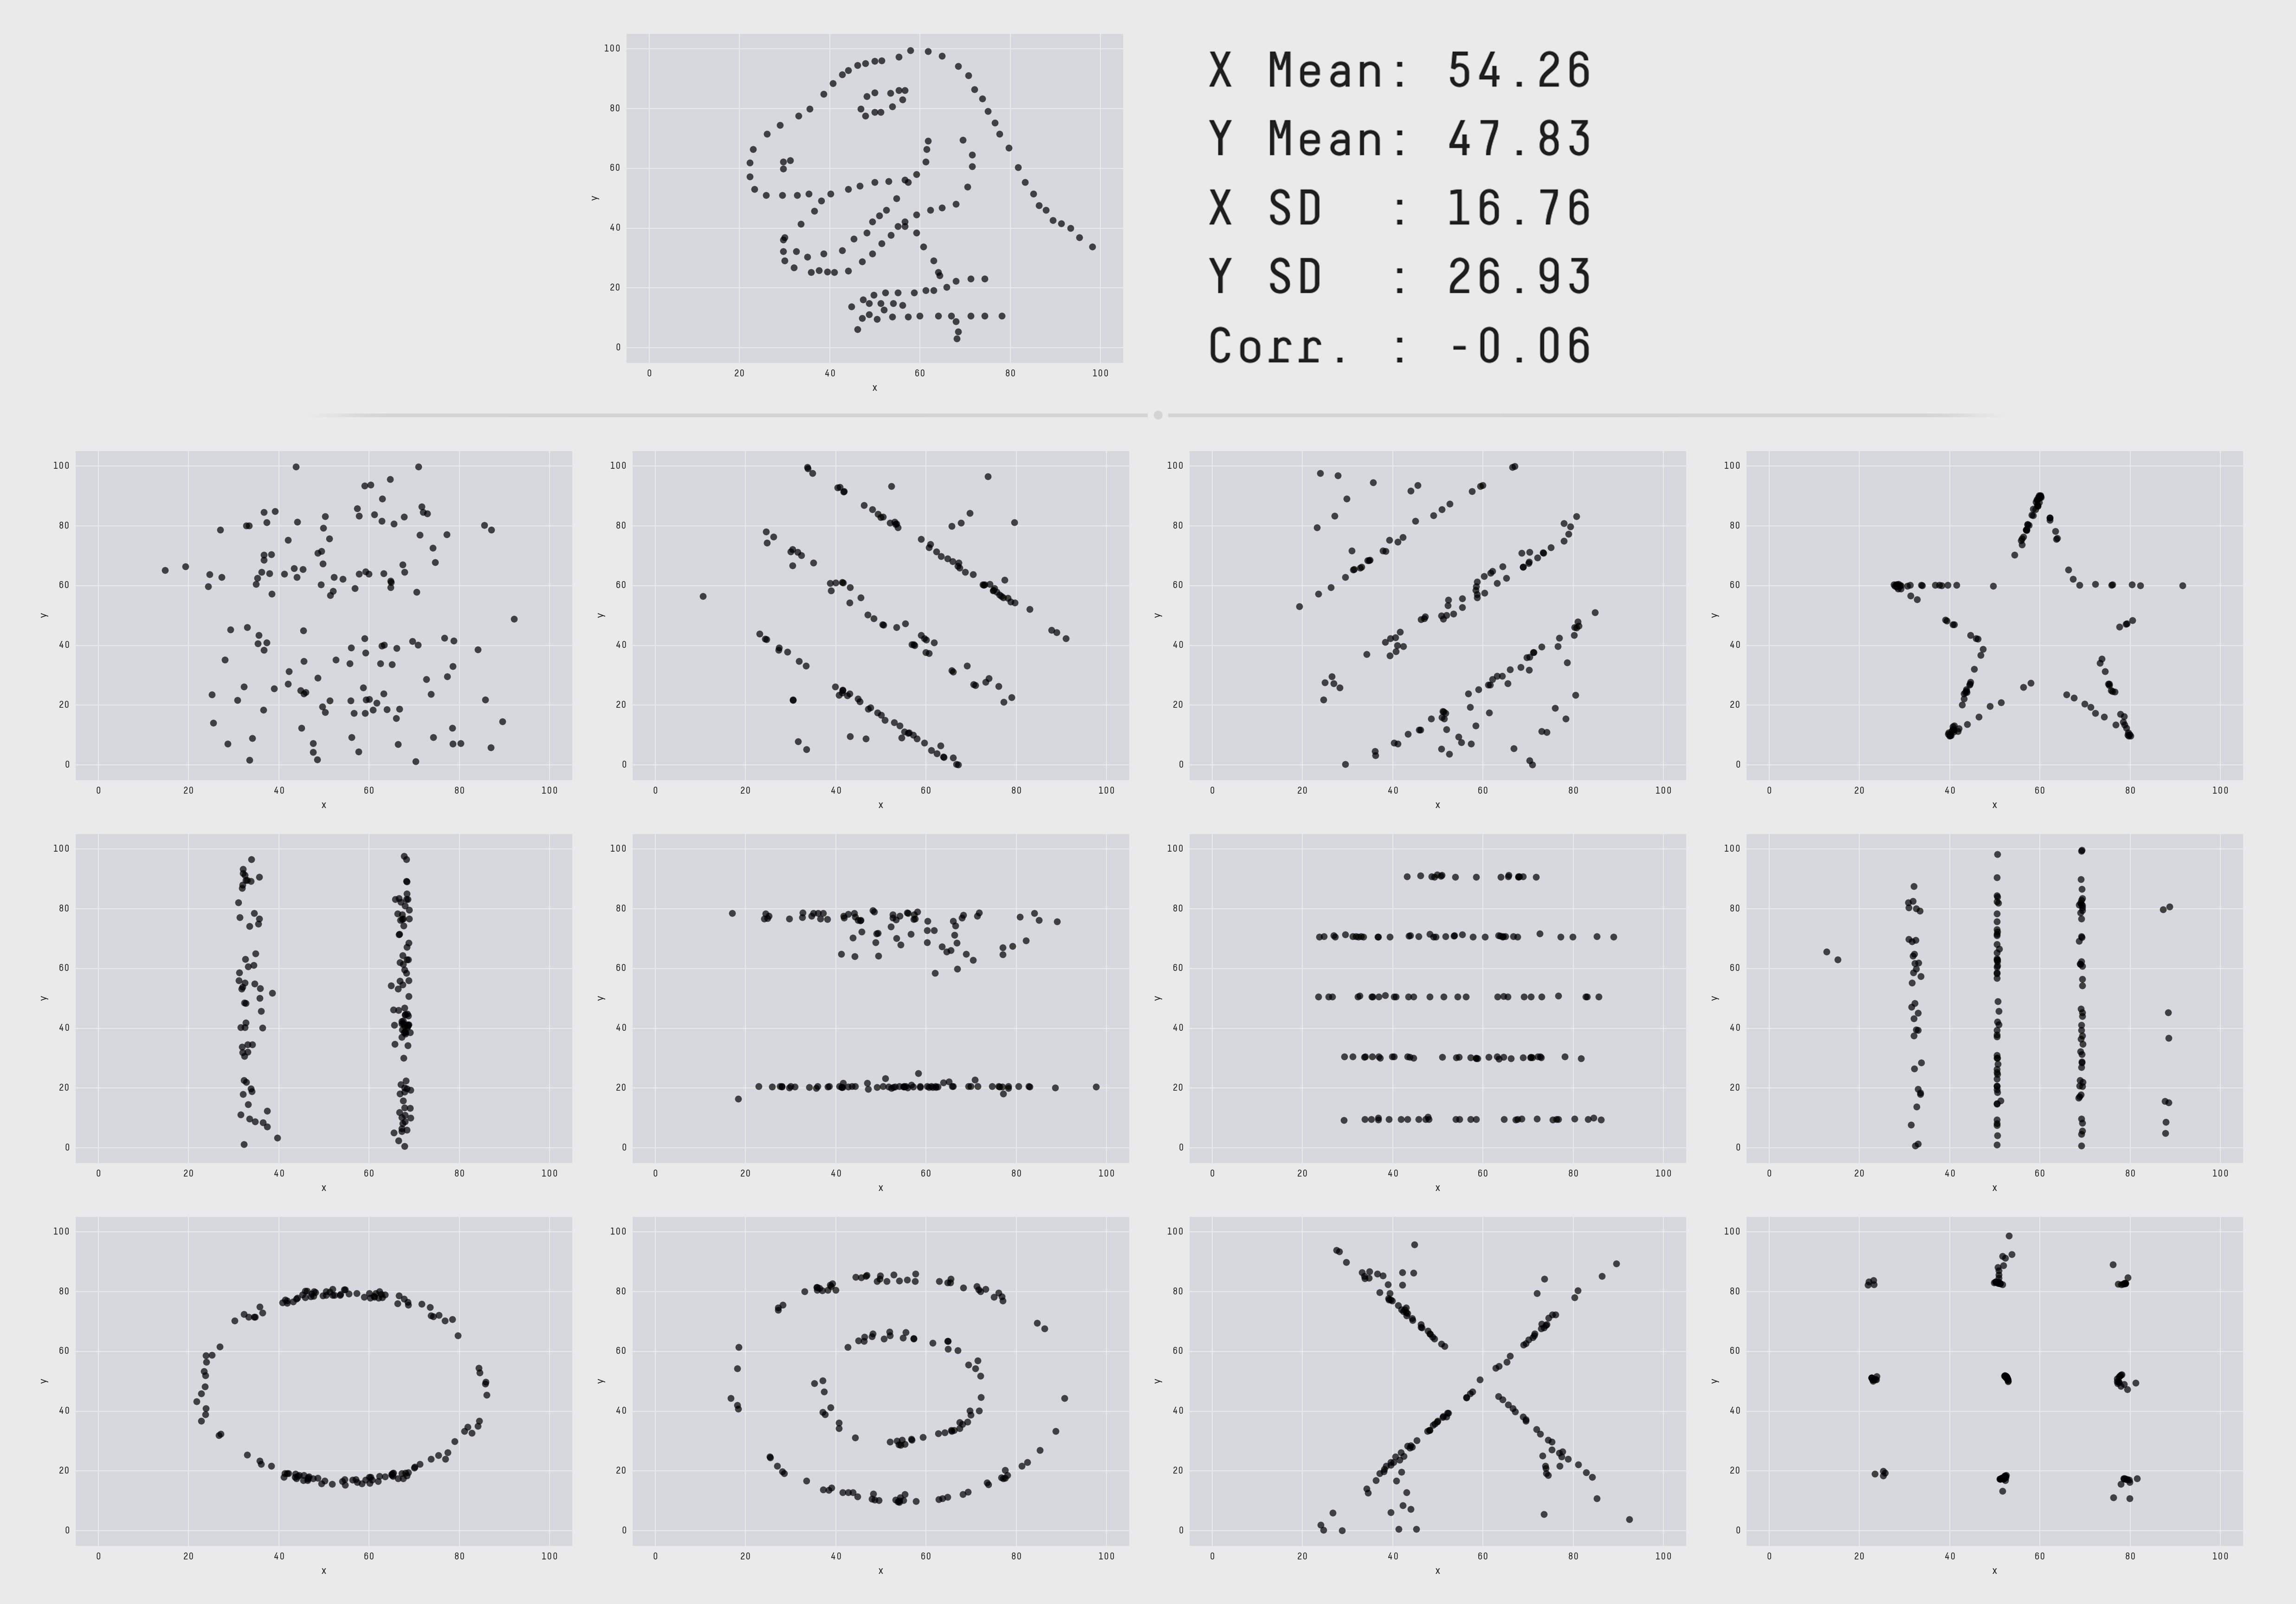
\includegraphics{datasaurus_alberto_cairo.png}
\caption{}
\end{figure}

This is why it's important to be aware of the underlying distribution of
data, and to not simply rely on summary statistics. Bar plots only show
summary statistics, and can thus hide potentially important differences
between groups.

    \subsection{Box plot}\label{box-plot}

One type of plot that \emph{does} reflect properties of distributions is
the box plot, or box-and-whiskers plot. It quite literally is two
stacked boxes with whiskers on either side. Each element of the plot
represents a quartile of the data (that's 25\% of the observations).
This type of plot thus tells you about each group's median (the 50th
percentile lies between the second and third quartile), and gives you a
rough idea of what the distribution looks like. Some boxplots also
include 'fliers': Values that lie outside the typical range, and could
be outliers.

Let's draw box plots for our two groups:

    \begin{Verbatim}[commandchars=\\\{\}]
{\color{incolor}In [{\color{incolor}34}]:} \PY{c+c1}{\PYZsh{} Draw a box for values from group x and group y. You can pass both }
         \PY{c+c1}{\PYZsh{} variables at the same time by combining them into a list, i.e. as}
         \PY{c+c1}{\PYZsh{} [x,y]. The same is true for the labels you would like to associate}
         \PY{c+c1}{\PYZsh{} with the groups.}
         \PY{n}{pyplot}\PY{o}{.}\PY{n}{boxplot}\PY{p}{(}\PY{p}{[}\PY{n}{x}\PY{p}{,}\PY{n}{y}\PY{p}{]}\PY{p}{,} \PY{n}{labels}\PY{o}{=}\PY{p}{[}\PY{l+s+s2}{\PYZdq{}}\PY{l+s+s2}{Group X}\PY{l+s+s2}{\PYZdq{}}\PY{p}{,}\PY{l+s+s2}{\PYZdq{}}\PY{l+s+s2}{Group Y}\PY{l+s+s2}{\PYZdq{}}\PY{p}{]}\PY{p}{)}
\end{Verbatim}


\begin{Verbatim}[commandchars=\\\{\}]
{\color{outcolor}Out[{\color{outcolor}34}]:} \{'boxes': [<matplotlib.lines.Line2D at 0x7f58b7f0aa90>,
           <matplotlib.lines.Line2D at 0x7f58b7f22450>],
          'caps': [<matplotlib.lines.Line2D at 0x7f58b7f18450>,
           <matplotlib.lines.Line2D at 0x7f58b7f18850>,
           <matplotlib.lines.Line2D at 0x7f58b7eac0d0>,
           <matplotlib.lines.Line2D at 0x7f58b7eac4d0>],
          'fliers': [<matplotlib.lines.Line2D at 0x7f58b7f22090>,
           <matplotlib.lines.Line2D at 0x7f58b7eaccd0>],
          'means': [],
          'medians': [<matplotlib.lines.Line2D at 0x7f58b7f18c50>,
           <matplotlib.lines.Line2D at 0x7f58b7eac8d0>],
          'whiskers': [<matplotlib.lines.Line2D at 0x7f58b7f0ab50>,
           <matplotlib.lines.Line2D at 0x7f58b7f18050>,
           <matplotlib.lines.Line2D at 0x7f58b7f22890>,
           <matplotlib.lines.Line2D at 0x7f58b7f22c90>]\}
\end{Verbatim}
            
    \begin{center}
    \adjustimage{max size={0.9\linewidth}{0.9\paperheight}}{output_28_1.png}
    \end{center}
    { \hspace*{\fill} \\}
    
    This is a pretty good visualisation of the two groups. We can see their
central tendency, because the median is represented by the coloured
horizontal line. In addition, we can see how observations are spread
out. For group \texttt{x}, all quartiles are roughly equally big, which
demonstrates that the data is uniformly distributed. For group
\texttt{y}, we can see that the second and third quartile (the boxes)
are smaller than the first and fourth quartile (the whiskers). This
illustrates that the distribution is denser around the median.

What we still can't see from the current plot is what the shape of the
distribution is. For example, it seems like group \texttt{y} is a normal
distribution, but it could also be that all values within the second and
third quartile are the same. For example, they could all be -0.5 and
0.5, and it would result in the same box plot.

    \subsection{Violin plot}\label{violin-plot}

Where box plots do not typically reveal the exact shape of a
distribution, violin plots are designed to do exactly that. They apply a
\emph{kernel density estimate} to characterise the shape of a
distribution, and plot that instead of boxes and whiskers. Fliers are
still denoted with a different marker (although what is considered a
"flier" can differ between box plots and violin plots, or more
accurately, per what standards are set within the function to draw the
plots).

Let's see what a violin plot of our two groups would look like:

    \begin{Verbatim}[commandchars=\\\{\}]
{\color{incolor}In [{\color{incolor}35}]:} \PY{c+c1}{\PYZsh{} Draw a violin plot for values from group x and group y. As }
         \PY{c+c1}{\PYZsh{} with the box plot, you can pass both variables at the same}
         \PY{c+c1}{\PYZsh{} time by combining them into a list, i.e. as [x,y].}
         \PY{n}{pyplot}\PY{o}{.}\PY{n}{violinplot}\PY{p}{(}\PY{p}{[}\PY{n}{x}\PY{p}{,}\PY{n}{y}\PY{p}{]}\PY{p}{,} \PY{n}{showmeans}\PY{o}{=}\PY{n+nb+bp}{True}\PY{p}{)}
\end{Verbatim}


\begin{Verbatim}[commandchars=\\\{\}]
{\color{outcolor}Out[{\color{outcolor}35}]:} \{u'bodies': [<matplotlib.collections.PolyCollection at 0x7f58b7e9e2d0>,
           <matplotlib.collections.PolyCollection at 0x7f58b7e9e5d0>],
          u'cbars': <matplotlib.collections.LineCollection at 0x7f58b7e2c210>,
          u'cmaxes': <matplotlib.collections.LineCollection at 0x7f58b7e9eb50>,
          u'cmeans': <matplotlib.collections.LineCollection at 0x7f58b7e9e1d0>,
          u'cmins': <matplotlib.collections.LineCollection at 0x7f58b7e9ee90>\}
\end{Verbatim}
            
    \begin{center}
    \adjustimage{max size={0.9\linewidth}{0.9\paperheight}}{output_31_1.png}
    \end{center}
    { \hspace*{\fill} \\}
    
    As you can see, the violin plot gives a much clearer picture of the
actual distribution of your data.

    \section{Choosing a visualisation
type}\label{choosing-a-visualisation-type}

As you have seen, different types of data visualisations exist, and each
come with their own benefits and downsides. Bar plots can be easily
understood, but also give you very little information about what the
data underlying an average looks like. In addition, whether or not it
makes sense to draw a bar highly depends on what kind of data you're
visualising. Adding error bars to bar plots to indicate the standard
error of the mean tells you something about the sampling process,
whereas adding error bars to indicate the standard deviation tells you
something about the sample.

If you're interested in visualising distributions in a more detailed
way, you could turn to box or violin plots. These provide a clearer
picture of what your data look like, and are still quite easy to
interpret.

What the best type of plot is depends on the data, and on what message
you would like your graph to illustrate. If you're simply saying "these
groups have different means", a bar plot with error bars that indicate
the standard error of the mean could work very well. However, if you're
trying to illustrate that two groups are from distributions with
different properties, you might need to turn to box or violin plots.

Finally, you are free to combine plots and types of visualisations. For
example, you could simply throw everything into one combined plot:

    \begin{Verbatim}[commandchars=\\\{\}]
{\color{incolor}In [{\color{incolor}36}]:} \PY{c+c1}{\PYZsh{} Determine the positions of the two groups\PYZsq{} visualisations}
         \PY{c+c1}{\PYZsh{} on the x\PYZhy{}axis.}
         \PY{n}{pos} \PY{o}{=} \PY{p}{[}\PY{l+m+mf}{0.5}\PY{p}{,} \PY{l+m+mf}{1.5}\PY{p}{]}
         
         \PY{c+c1}{\PYZsh{} Draw violin plots for each group, but don\PYZsq{}t draw the mean,}
         \PY{c+c1}{\PYZsh{} median, or extrema.}
         \PY{n}{vplot} \PY{o}{=} \PY{n}{pyplot}\PY{o}{.}\PY{n}{violinplot}\PY{p}{(}\PY{p}{[}\PY{n}{x}\PY{p}{,}\PY{n}{y}\PY{p}{]}\PY{p}{,} \PY{n}{positions}\PY{o}{=}\PY{n}{pos}\PY{p}{,} \PYZbs{}
             \PY{n}{showmeans}\PY{o}{=}\PY{n+nb+bp}{False}\PY{p}{,} \PY{n}{showmedians}\PY{o}{=}\PY{n+nb+bp}{False}\PY{p}{,} \PY{n}{showextrema}\PY{o}{=}\PY{n+nb+bp}{False}\PY{p}{)}
         \PY{c+c1}{\PYZsh{} Set the colour of the violin plot.}
         \PY{k}{for} \PY{n}{violin} \PY{o+ow}{in} \PY{n}{vplot}\PY{p}{[}\PY{l+s+s2}{\PYZdq{}}\PY{l+s+s2}{bodies}\PY{l+s+s2}{\PYZdq{}}\PY{p}{]}\PY{p}{:}
             \PY{n}{violin}\PY{o}{.}\PY{n}{set\PYZus{}color}\PY{p}{(}\PY{l+s+s2}{\PYZdq{}}\PY{l+s+s2}{\PYZsh{}FF69B4}\PY{l+s+s2}{\PYZdq{}}\PY{p}{)}
         \PY{c+c1}{\PYZsh{} Draw box plots for each groups on the same positions.}
         \PY{n}{bplot} \PY{o}{=} \PY{n}{pyplot}\PY{o}{.}\PY{n}{boxplot}\PY{p}{(}\PY{p}{[}\PY{n}{x}\PY{p}{,}\PY{n}{y}\PY{p}{]}\PY{p}{,} \PY{n}{positions}\PY{o}{=}\PY{n}{pos}\PY{p}{,} \PYZbs{}
             \PY{n}{labels}\PY{o}{=}\PY{p}{[}\PY{l+s+s2}{\PYZdq{}}\PY{l+s+s2}{Group X}\PY{l+s+s2}{\PYZdq{}}\PY{p}{,} \PY{l+s+s2}{\PYZdq{}}\PY{l+s+s2}{Group Y}\PY{l+s+s2}{\PYZdq{}}\PY{p}{]}\PY{p}{)}
         \PY{c+c1}{\PYZsh{} Set the colour of horizontal lines that indicate the median}
         \PY{c+c1}{\PYZsh{} in each box plot.}
         \PY{k}{for} \PY{n}{line} \PY{o+ow}{in} \PY{n}{bplot}\PY{p}{[}\PY{l+s+s2}{\PYZdq{}}\PY{l+s+s2}{medians}\PY{l+s+s2}{\PYZdq{}}\PY{p}{]}\PY{p}{:}
             \PY{n}{line}\PY{o}{.}\PY{n}{set\PYZus{}color}\PY{p}{(}\PY{l+s+s2}{\PYZdq{}}\PY{l+s+s2}{\PYZsh{}FF69B4}\PY{l+s+s2}{\PYZdq{}}\PY{p}{)}
         
         \PY{c+c1}{\PYZsh{} Finally, draw the individual data points for each group. The}
         \PY{c+c1}{\PYZsh{} points need to be plotted to the right of each of the }
         \PY{c+c1}{\PYZsh{} box/violin plots. To do so, we first need to create two }
         \PY{c+c1}{\PYZsh{} vectors that code for the position of each sample from each }
         \PY{c+c1}{\PYZsh{} group on the x\PYZhy{}axis.}
         \PY{n}{x\PYZus{}pos} \PY{o}{=} \PY{n}{numpy}\PY{o}{.}\PY{n}{ones}\PY{p}{(}\PY{n}{x}\PY{o}{.}\PY{n}{shape}\PY{p}{)} \PY{o}{*} \PY{n}{pos}\PY{p}{[}\PY{l+m+mi}{0}\PY{p}{]} \PY{o}{+} \PY{l+m+mf}{0.3}
         \PY{n}{y\PYZus{}pos} \PY{o}{=} \PY{n}{numpy}\PY{o}{.}\PY{n}{ones}\PY{p}{(}\PY{n}{y}\PY{o}{.}\PY{n}{shape}\PY{p}{)} \PY{o}{*} \PY{n}{pos}\PY{p}{[}\PY{l+m+mi}{1}\PY{p}{]} \PY{o}{+} \PY{l+m+mf}{0.3}
         \PY{c+c1}{\PYZsh{} Then, we simply need to plot the samples. The alpha keyword}
         \PY{c+c1}{\PYZsh{} indicates the transparancy of each sample.}
         \PY{n}{pyplot}\PY{o}{.}\PY{n}{plot}\PY{p}{(}\PY{n}{x\PYZus{}pos}\PY{p}{,} \PY{n}{x}\PY{p}{,} \PY{l+s+s1}{\PYZsq{}}\PY{l+s+s1}{.}\PY{l+s+s1}{\PYZsq{}}\PY{p}{,} \PY{n}{color}\PY{o}{=}\PY{l+s+s2}{\PYZdq{}}\PY{l+s+s2}{\PYZsh{}FF69B4}\PY{l+s+s2}{\PYZdq{}}\PY{p}{,} \PY{n}{alpha}\PY{o}{=}\PY{l+m+mf}{0.1}\PY{p}{)}
         \PY{n}{pyplot}\PY{o}{.}\PY{n}{plot}\PY{p}{(}\PY{n}{y\PYZus{}pos}\PY{p}{,} \PY{n}{y}\PY{p}{,} \PY{l+s+s1}{\PYZsq{}}\PY{l+s+s1}{.}\PY{l+s+s1}{\PYZsq{}}\PY{p}{,} \PY{n}{color}\PY{o}{=}\PY{l+s+s2}{\PYZdq{}}\PY{l+s+s2}{\PYZsh{}FF69B4}\PY{l+s+s2}{\PYZdq{}}\PY{p}{,} \PY{n}{alpha}\PY{o}{=}\PY{l+m+mf}{0.1}\PY{p}{)}
\end{Verbatim}


\begin{Verbatim}[commandchars=\\\{\}]
{\color{outcolor}Out[{\color{outcolor}36}]:} [<matplotlib.lines.Line2D at 0x7f58b7f52c10>]
\end{Verbatim}
            
    \begin{center}
    \adjustimage{max size={0.9\linewidth}{0.9\paperheight}}{output_34_1.png}
    \end{center}
    { \hspace*{\fill} \\}
    

    % Add a bibliography block to the postdoc
    
    
    
    \end{document}
